\documentclass{article}

\usepackage{parskip}
\usepackage{graphicx}
\usepackage{float}

\begin{document}

\section{Architectural Patterns}

An architectural pattern is a general, reusable solution to a
commonly occurring problem in software architecture within a
given context.

It comprises of:
\begin{itemize}
\item
  \textbf{Context} that provides a frame for a problem.
\item
  \textbf{Problem} that is a generalized description of a class of problems with
  QA requirements that need to be met.
\item
  \textbf{Solution} that is suitably generalized in the same way as the problem.
\end{itemize}


We consider:
\begin{itemize}
\item
  \textbf{Static Patterns} designed to solve issues around development and maintenance of
  the code bae.
\item
  \textbf{Connector and component models} that consider patterns of interaction,
  monitoring at runtime and responses to stimuli.
\item
  \textbf{Deployment patterns} that consider the allocation of elements to hardware
  resources and the availability of resources in the system.
\end{itemize}

\subsection{Static Patterns}
\subsubsection{Layer Pattern}

Description:
% IMAGE: Pipes
\begin{figure}[H]
\centering
  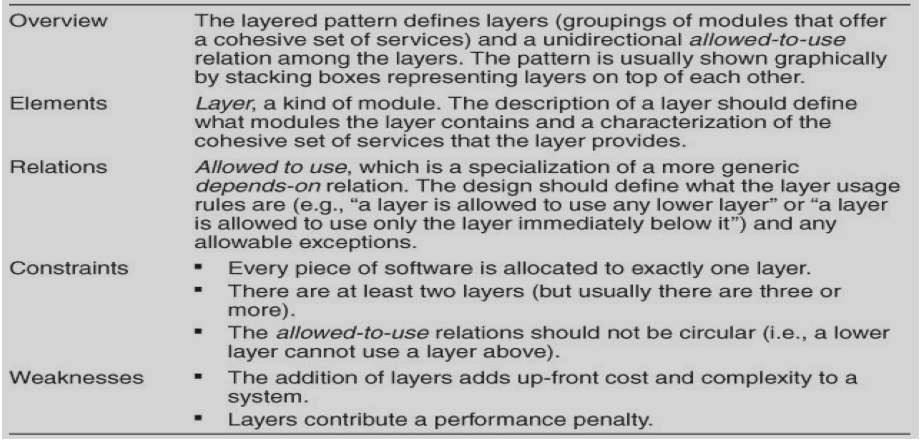
\includegraphics[width=1\linewidth]{images/layered.png}
%\caption{-}
\end{figure}


In a logical multilayered architecture for an
information system with an object-oriented design,
the following four are the most common:

\begin{itemize}
\item
  Presentation layer (a.k.a UI layer, view layer ...)
\item
  Application layer (a.k.a service layer)
\item
  Business layer (a.k.a business logical layer (BLL), domain layer)
\item
  Data access layer (a.k.a persistence layer, logging, networking, database)
\end{itemize}

% IMAGE: Pipes
\begin{figure}[H]
\centering
  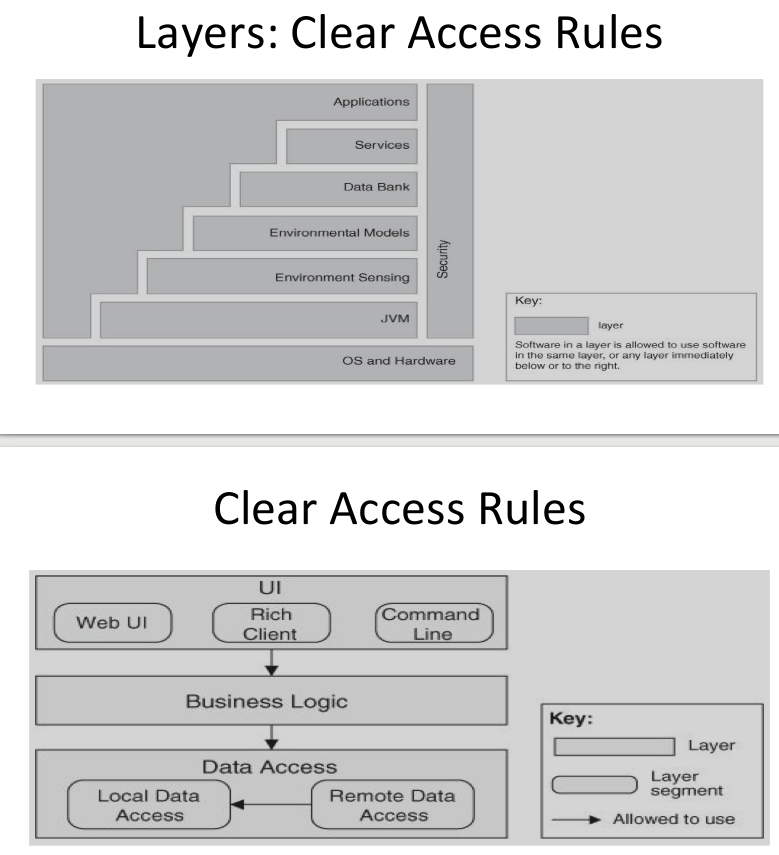
\includegraphics[width=1\linewidth]
  {images/access_rules.png}
%\caption{-}
\end{figure}

\subsection{Connector and component models}

\subsubsection{Model-View-Controller}

\textbf{Context}: The user interface is subject to continuing change to either
meet the needs of the application or diversity in the user group.

\textbf{Problem}:
\begin{itemize}
\item
  Isolating the UI functionality from the Application functionality.
\item
  Maintaining multiple views in the presence of change in the underlying data.
\end{itemize}


% IMAGE: Pipes
\begin{figure}[H]
\centering
  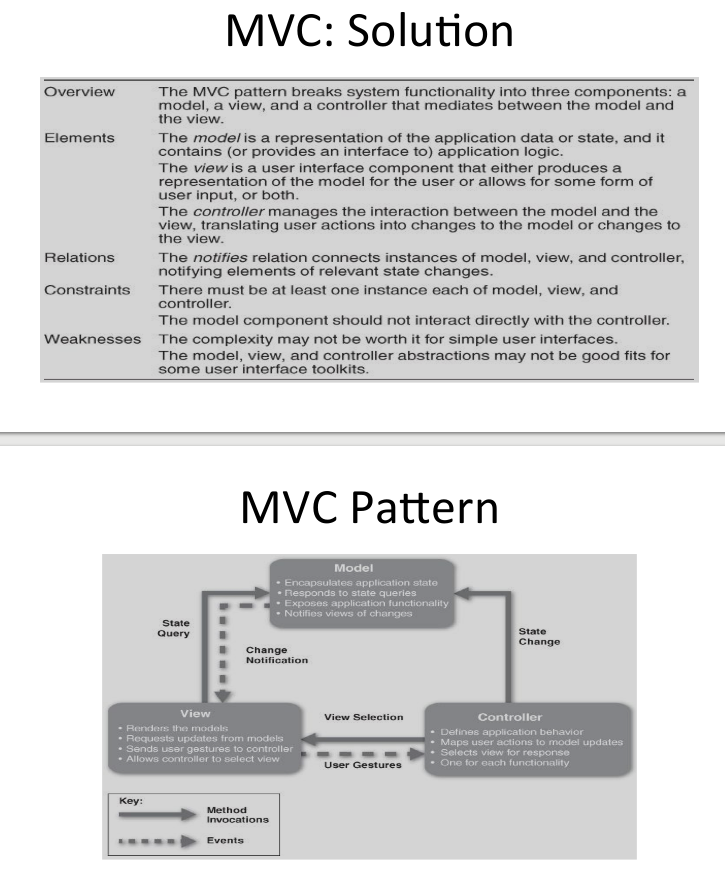
\includegraphics[width=1\linewidth]
  {images/mvc.png}
%\caption{-}
\end{figure}

\subsection{Deployment/Allocation patterns}

% Context:
% \begin{itemize}
% \item
%   We are concerned with resource use.
% \item
%   We consider flexible deployment of resource.
% \item
%   the QAs we care about are sensitive to the pattern of deployment and the use
%   of resources.
% \end{itemize}

\subsubsection{Map-reduce pattern}

Context:
\begin{itemize}
\item
  We have large quantities of data that we want to process in parallel.
\item
  This encourages an approach that involves significant amounts of independent processing.
\end{itemize}

% IMAGE: Pipes
\begin{figure}[H]
\centering
  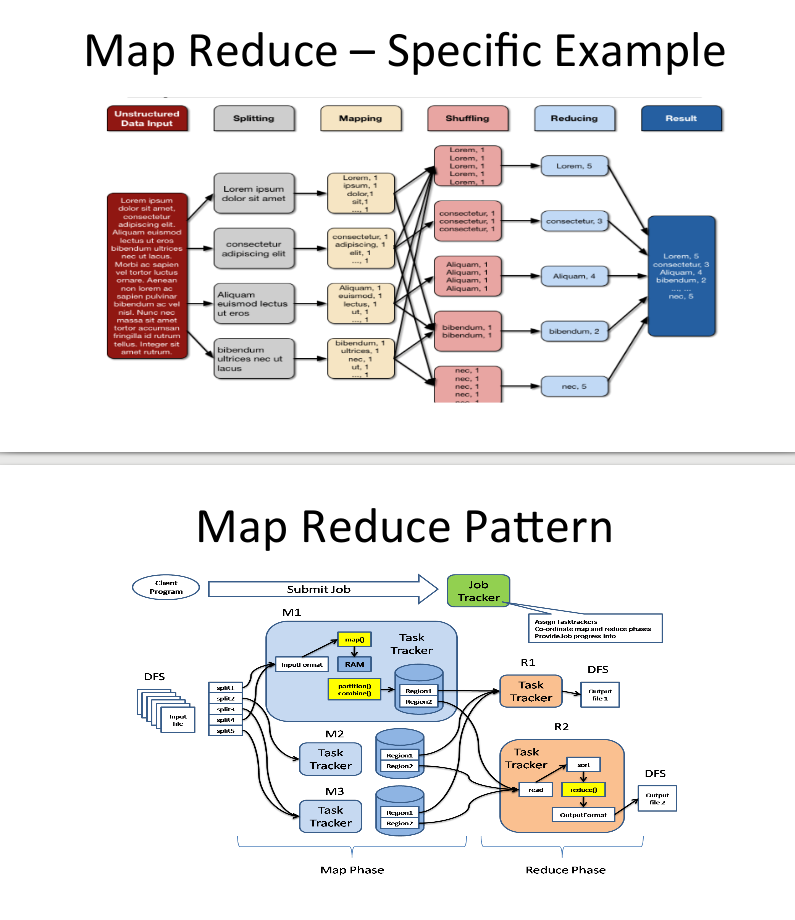
\includegraphics[width=1\linewidth]
  {images/mapreduce.png}
%\caption{-}
\end{figure}

\subsubsection{Other Allocation Patterns}

\begin{itemize}
\item
  Multi-tier architecture pattern
\item
  Cloud architectures
\end{itemize}

\subsection{Other patterns}
\begin{itemize}
\item
  Pipe and Filter Pattern
\item
  Broker Pattern
\item
  Client-Server Pattern
\item
  Peer-to-Peer Pattern
\item
  Service-Oriented Architecture Pattern
\item
  Publish-Subscribe Pattern
\item
  Shared Data Pattern
\end{itemize}

\section{Relationship between Patterns and Tactics}

% IMAGE: Pipes
\begin{figure}[H]
\centering
  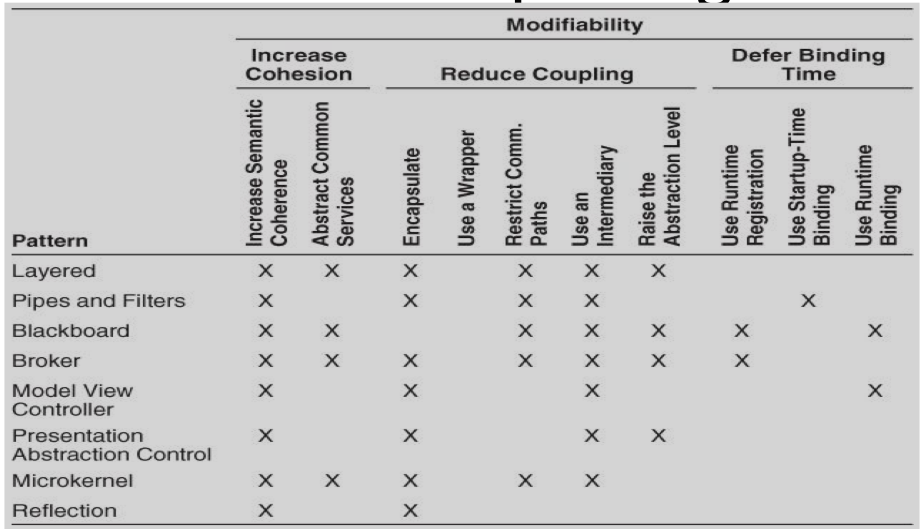
\includegraphics[width=1\linewidth]
  {images/relationship.png}
%\caption{-}
\end{figure}

\end{document}